
\documentclass[final]{beamer}

\usetheme{RJH}
\usepackage[utf8]{inputenc}
\usepackage[frenchb]{babel}
\usepackage[orientation=landscape,size=a2,scale=1.2]{beamerposter}
\usepackage[absolute,overlay]{textpos}
\usepackage{url}
\usepackage{graphicx}
\graphicspath{{./images/}}
% \usepackage{xcolor}
% \usepackage{xspace}
\usepackage{hyperref}
\usepackage{amsmath}
\usepackage{amssymb}
\usepackage[labelformat=empty]{caption}
\usepackage{framed}
\usepackage{wrapfig}
\usepackage{minted}
\usepackage{xspace}


\definecolor{rulecolor}{rgb}{0.80,0.80,0.80}
\newminted{python}{frame=single,rulecolor=\color{rulecolor}}

\setlength{\TPHorizModule}{\paperwidth}
\setlength{\TPVertModule}{\paperheight}

\newcommand{\qedwhite}{\hfill \ensuremath{\Box}}

\definecolor{lightgreen}{rgb}{0.0,0.8,0.0}
\definecolor{lightblue}{rgb}{0.3,0.8,1.0}
\definecolor{lightred}{rgb}{0.874,0.180,0.105}
\definecolor{gray}{rgb}{0.4,0.4,0.4}
\definecolor{lightgray}{rgb}{0.8,0.8,0.8}
\definecolor{shadecolor}{rgb}{0.9,0.9,0.9}

\newcommand{\sklearn}{\textit{scikit-learn}\xspace}


\title{Scikit-Learn: Machine Learning in the Python ecosystem}
\author{Arnaud Joly, Gilles Louppe, \textit{and all \sklearn contributors}\\[1.5ex]
{\tiny

\includegraphics[scale=0.16]{mail}~\url{a.joly@ulg.ac.be}

\includegraphics[scale=0.6]{twitter}~\href{https://twitter.com/JolyArnaud}{@JolyArnaud}

\includegraphics[scale=0.16]{mail}~\url{g.louppe@ulg.ac.be}

\includegraphics[scale=0.6]{twitter}~\href{https://twitter.com/glouppe}{@glouppe}
~~~\url{http://scikit-learn.org}
}
}

\footer{}
\date{}

\makeatletter
\newcommand{\superimpose}[2]{%
  {\ooalign{$#1\@firstoftwo#2$\cr\hfil$#1\@secondoftwo#2$\hfil\cr}}}
\makeatother

\begin{document}
\begin{frame}[fragile]


%% Column 1 ==================================================================

\begin{textblock}{0.32}(0.01,0.14)


% \begin{block}{Abstract \phantom{p}}
% The scikit-learn (\url{http://scikit-learn.org}) project is an increasingly popular
% machine learning library written in Python. It is designed to be simple and
% efficient, useful to both experts and non-experts, and reusable in a variety of
% contexts. The primary aim of the project is to provide a compendium of
% efficient implementations of classic, well-established machine learning
% algorithms.
% Among other things, it includes classical supervised and
% unsupervised learning algorithms, tools for model evaluation and selection,
% as well as tools for data preprocessing and feature engineering. Scikit-learn
% is distributed under the 3-clause BSD license, encouraging its free use in
% both commercial and academic settings.

% \vspace{0.3cm}

% This presentation will illustrate the use of scikit-learn as a component of the
% larger scientific Python environment to solve complex data analysis tasks.
% Examples will include end-to-end workflows based on powerful
% and popular algorithms in the library. Among others, we will show how to
% explore some biological data using random forest.

% \vspace{0.3cm}

% The library is widely used in the Bioinformatics and Modelling research unit.
% \end{block}

% \vspace{0.5cm}

\begin{block}{Overview \phantom{p}}
\begin{columns}
\begin{column}{0.01\textwidth}
\end{column}
\begin{column}{0.3\textwidth}
\begin{center}

\includegraphics[width=\textwidth]{sklearn-logo}
\end{center}
\end{column}
\begin{column}{0.69\textwidth}
The \sklearn project is an increasingly
popular machine learning library written in Python. It is designed to be
\textbf{simple and efficient}, useful to both experts and non-experts, and
reusable in a variety of contexts. The
primary aim of the project is to provide a compendium of
efficient implementations of classic, well-established machine learning
algorithms.
\end{column}
\end{columns}

\vspace{0.3cm}

\textbf{\structure{Supervised learning:}} linear models
(ridge, lasso, elastic net, \ldots), ensemble methods
(random forests, bagging, boosting, \ldots), support vector machines.


\begin{center}
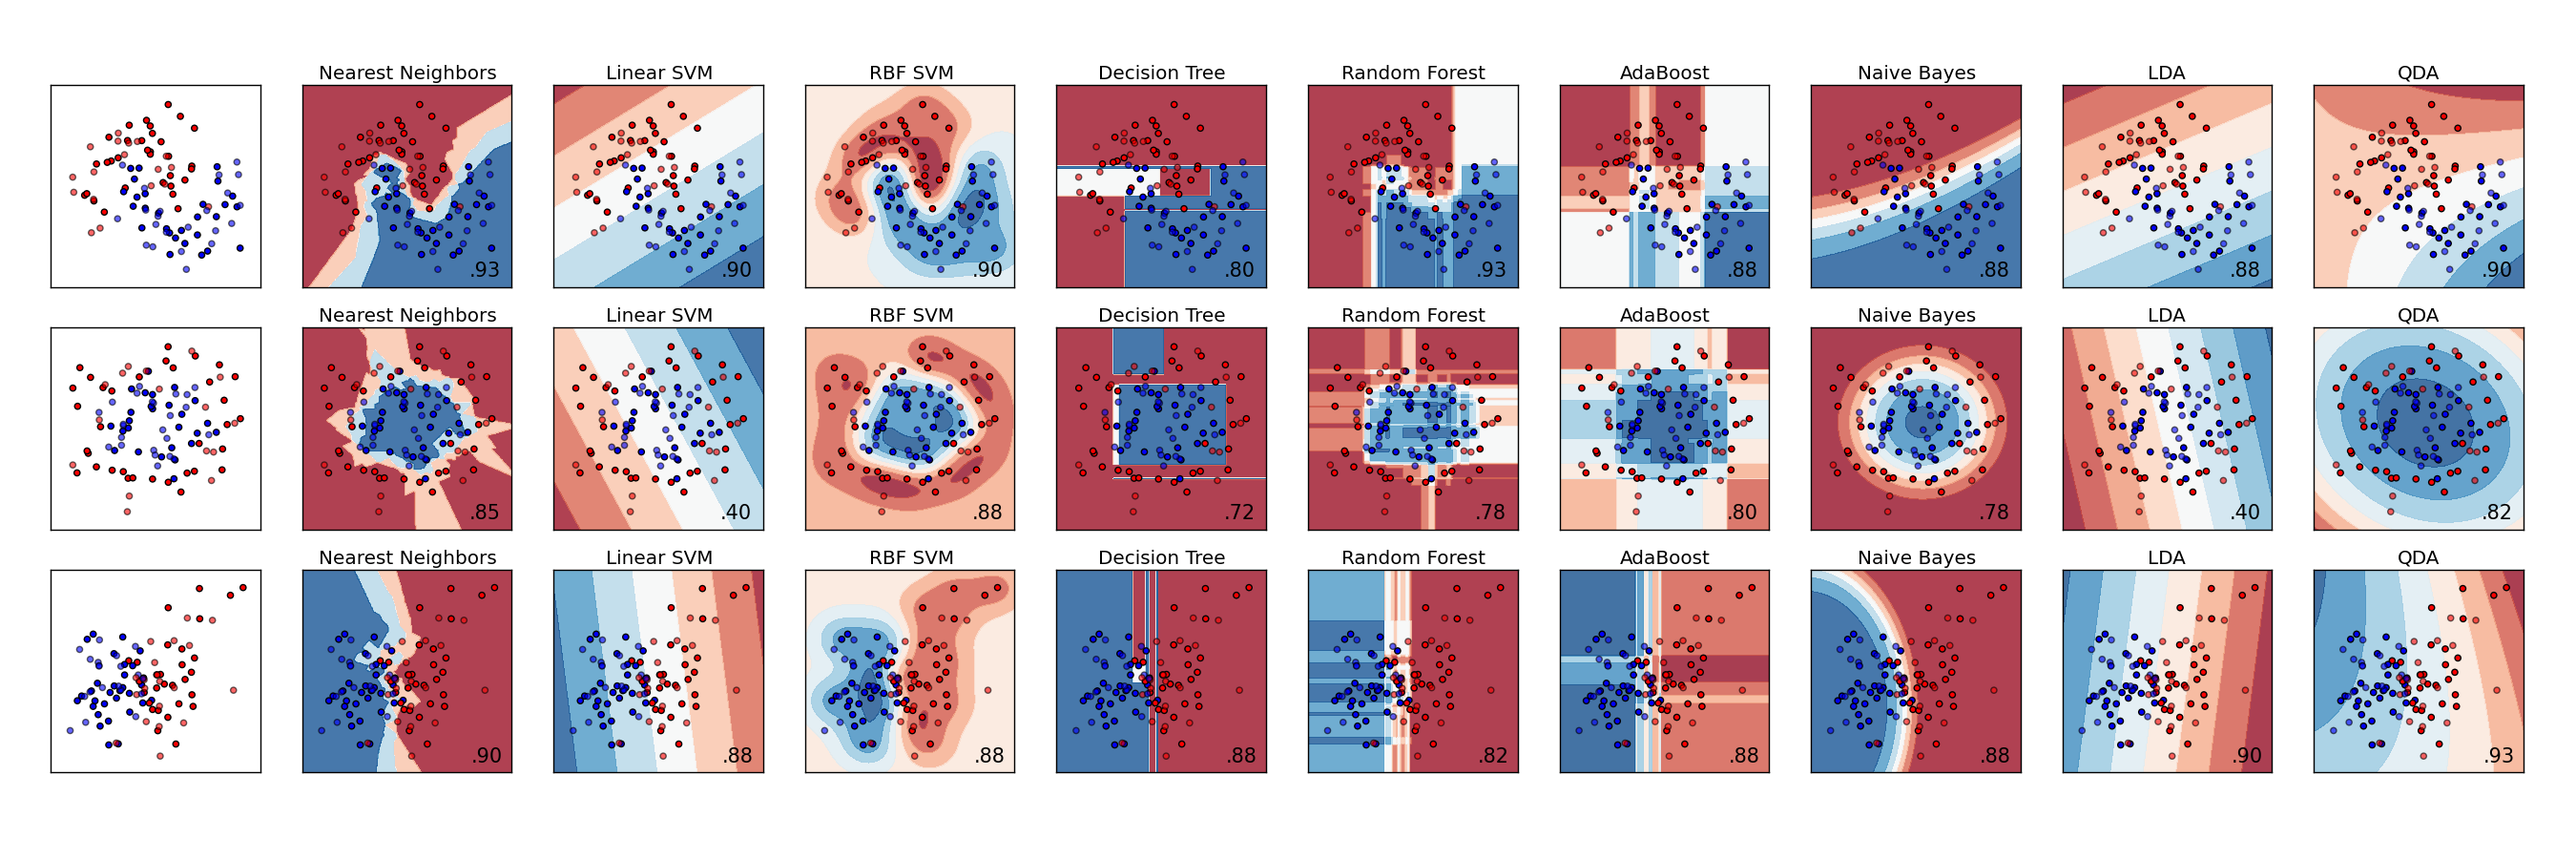
\includegraphics[width=\textwidth]{comparison}
\end{center}

\textbf{\structure{Unsupervised learning:}} clustering (KMeans, Ward, ...),
matrix decomposition (PCA, ICA, \ldots), outlier detection.

\vspace{0.3cm}

\textbf{\structure{Model selection and evaluation:}} cross-validation,
grid-search, lots of metrics.

\vspace{0.3cm}

\ldots and many more! (See our
\href{http://scikit-learn.org/stable/modules/classes.html}{Reference}).
\end{block}

\begin{block}{Collaborative development \phantom{p}}
Around 10 core developers
and more than 100 occasional contributors from all around the world.
All are working together on
\href{https://github.com/scikit-learn/scikit-learn}{GitHub} with strict coding
guidelines, including style consistency, unit-test coverage, documentation,
examples and code review.

\begin{columns}[b]
\begin{column}{0.01\textwidth}
\end{column}
\begin{column}{0.485\textwidth}
\begin{center}
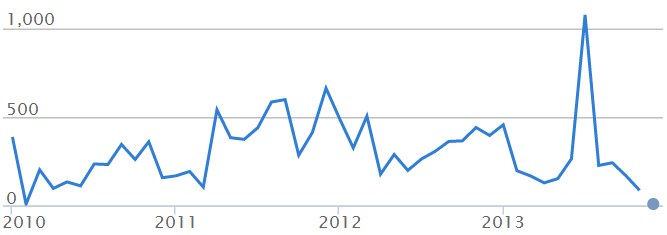
\includegraphics[width=\textwidth]{commits} \\
Number of commits\end{center}
\end{column}
\begin{column}{0.485\textwidth}
\begin{center}
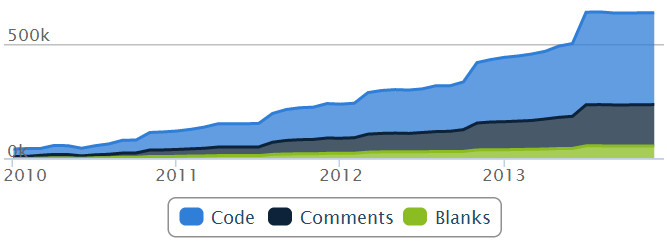
\includegraphics[width=\textwidth]{loc} \\
Number of line of codes
\end{center}
\end{column}
\end{columns}

\end{block}


\begin{block}{Who is using scikit-learn? \phantom{p}}

In the Bioinformatics and Modelling research unit, \sklearn is used by several
researchers to perform \textbf{gene interaction discovery},
\textbf{bioinformatics image analysis} such as in the Cytomine project or
more \textbf{fundamental research} in machine learning.
The research unit is also actively contributing to the library with two
researchers as core contributors.

\vspace{0.3cm}

In the applied science faculty of the University of Liège (ULg), \sklearn is
taught in the \textbf{machine learning course} and often used in students'
master's theses.

\vspace{0.3cm}

\sklearn is widely used in the industry (\emph{e.g.} Spotify, Evernote,
Phimeca) and in the academics world (\emph{e.g.} ULg, Inria,
Télécom ParisTech).
\end{block}

\end{textblock}



%% Column 2 ==================================================================

\begin{textblock}{0.32}(0.34,0.14)
\begin{block}{A simple and unified API \phantom{p}}

All objects in \sklearn share a \textbf{uniform and limited API}
consisting of three complementary interfaces:
\begin{itemize}
\item[-] an \structure{estimator} interface for building and fitting models;
\item[-] a \structure{predictor} interface for making predictions;
\item[-] a \structure{transformer} interface for converting data.
\end{itemize}
All of them takes as input data which is structured as \structure{Numpy} arrays
or \structure{Scipy} sparse matrices.
%\vspace{0.3cm}
% Experimenting with different learning algorithms is as simple as changing a
% class definition.
% Through composition interfaces (e.g., Pipeline and
% FeatureUnion), the library also offers powerful mechanisms to express a wide
% variety of learning tasks within a small amount of code.
\begin{pythoncode}
>>> # Load data
>>> from sklearn.datasets import load_digits
>>> data = load_digits()
>>> X, y = data.data, data.target

>>> # Instantiate a classifier
>>> from sklearn.tree import DecisionTreeClassifier # Change this
>>> clf = DecisionTreeClassifier()                  # ... and that

>>> # Do stuff (and rely on the common interface across estimators)
>>> from sklearn.pipeline import Pipeline
>>> from sklearn.decomposition import PCA
>>> pipeline = Pipeline([("pca", PCA()), ("classifier", clf)])

>>> # Validate the model
>>> from sklearn.cross_validation import cross_val_score
>>> print "Accuracy = ", cross_val_score(pipeline, X, y, cv=3).mean()
Accuracy = 0.796863873387
\end{pythoncode}

% >>> # Optimize model hyperparameters
% >>> from sklearn.grid_search import GridSearchCV
% >>> hyperparameters = {"pca__n_components": [10, 20, 40]}
% >>> estimator = GridSearchCV(pipeline, hyperparameters)

% \vspace{0.5cm}

% \sklearn integrates well with the the scientific Python ecosystem including
% NumPy for efficient manipulation of multi-dimensional arrays,
% SciPy for specialized data structures (e.g., sparse matrices) and
% lower-level scientific algorithms, IPython for interactive exploration,
% Matplotlib (for vizualization), \ldots

\end{block}

\begin{block}{Data analysis in Python \phantom{p}}

Let us illustrate the various components of the scientific Python ecosystem
for the analysis of scientific data. We consider genetic data from the HapMap
project which catalogs common genetic variants in human beings from 11 human
populations from different parts of the world.

% Challenges:
% \begin{itemize}
% \item[-] GBs of raw data from a large collection of genotype data files (one
%          per chromosome/population);
% \item[-] SNPs are sometimes missing for some individuals or an entire
%          populations;
% \item[-] Values are heterogeneous (numbers, strings, symbols).
% \end{itemize}

\vspace{0.3cm}

% \sklearn expects input data to be represented as two-dimensional
% \structure{NumPy} arrays of numerical values.
% In our case, the HapMap data is
% not represented in this way and needs to be preprocessed to conform to our
% standards.
% We can rely on \structure{pandas}, \structure{NumPy} or other battery included
% modules for loading, converting and merging a datafiles into a single NumPy array.

\structure{1) Data preprocessing with \sklearn and pandas}
\vspace{0.3cm}

\textbf{Loading, converting and merging raw data files} is easily done
using \sklearn, \structure{pandas}, \structure{NumPy} or other Python battery
included modules.

\vspace{0.3cm}

Once data are loaded, \sklearn and \structure{pandas}
provide \textbf{data preprocessing tools} to extract and to normalize data.
% It regroups genotypes for all SNPs (from all 23 chromosomes) reported by the
% HapMap genotyping centers.
For instance, there is missing values in the HapMap dataset that can be
inferred using the most frequent values associated to each SNP.
\begin{pythoncode}
>>> from sklearn.preprocessing import Imputer
>>> imputer = Imputer(strategy="most_frequent", missing_values=-1)
>>> X = imputer.fit_transform(X)
\end{pythoncode}

\vspace{0.3cm}
\structure{2) Data visualization with matplotlib}
\vspace{0.3cm}

In exploratory analysis, \textbf{data visualization} plays an important role in
identifying interesting patterns. However data are often high dimensional.
\sklearn implements several \textbf{dimensionality reduction methods}.
For illustration, let's study chromosome 15. First, we reduce
 the dimensionality of the data from 33800 to 2.
\begin{pythoncode}
>>> from sklearn.decomposition import RandomizedPCA
>>> Xp = RandomizedPCA(n_components=2).fit_transform(X)
\end{pythoncode}

\end{block}

\end{textblock}


%% Column 3 ==================================================================

\begin{textblock}{0.32}(0.67,0.14)
\begin{block}{\vspace*{-3ex}}

We rely on the \structure{matplotlib} module for generating our figures and
plots. In this plot, individuals from a same population are
clustered together, which confirms that they share the same genetic variants.

\begin{center}
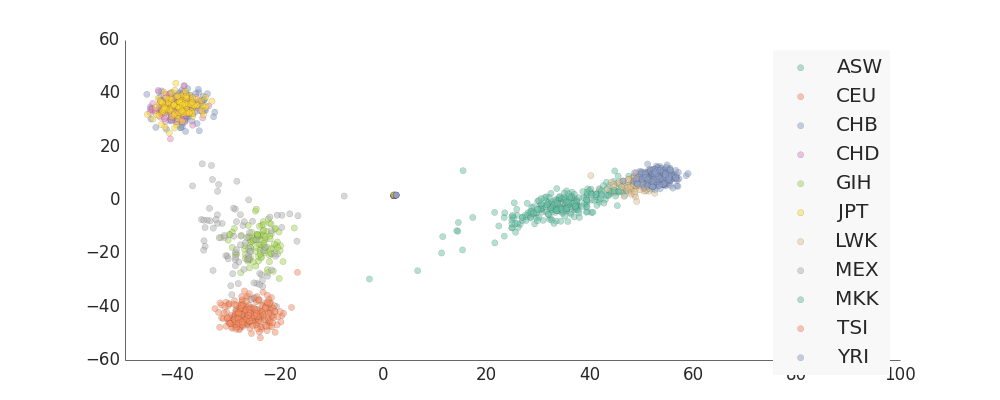
\includegraphics[width=0.6\textwidth]{randomized_pca} \\
\end{center}


\vspace{0.3cm}
\structure{3) Learning from the data with \sklearn}
\vspace{0.3cm}

In predictive analytics, the goal is to extract information to classify objects
or to predict continuous value. With \sklearn, you can \textbf{learn a model
from the data}. We consider the learning task that consists in predicting the population
of an individual given chromosome 15. Let us learn a forest of
randomized tree model.
\begin{pythoncode}
>>> from sklearn.cross_validation import train_test_split
>>> X_train, X_test, y_train, y_test = train_test_split(X, y)

>>> from sklearn.ensemble import ExtraTreesClassifier
>>> clf = ExtraTreesClassifier(n_estimators=100,
                               max_features=0.2).fit(X_train, y_train)

# Model prediction
>>> clf.predict(X_test)
array(['CHB', 'ASW', 'CEU', ..., 'GIH'])
\end{pythoncode}

\vspace{0.3cm}
\structure{4) Learning from a \sklearn model}
\vspace{0.3cm}

Once a model is fitted, you can \textbf{learn from the model}.
Let us now examine the importance associated to each SNP to predict
the population. The top SNP is rs1834640, which is known to be associated with
skin pigmentation.

\begin{center}
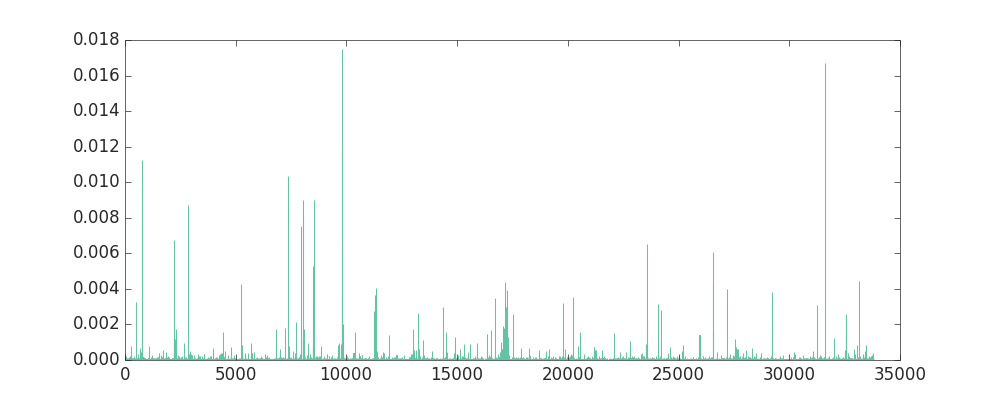
\includegraphics[width=0.6\textwidth]{extra_trees} \\
SNPs importance of chromosome 15
\end{center}

\end{block}

\begin{block}{Conclusions  \phantom{p}}

Python data-oriented packages tend to complement and integrate smoothly with
each other. Together, they provide a powerful, flexible and coherent working
environment for real-world scientific data analysis. Python is good and
viable replacement to Matlab and R.

\vspace{0.3cm}

Scikit-Learn complements this ecosystem with machine learning algorithms and
data analysis utilities.

\begin{center}
\begin{large}
\url{www.scikit-learn.org}
\end{large}
\end{center}
\end{block}

\end{textblock}


\end{frame}
\end{document}
